	\documentclass[conference]{IEEEtranl}
	\makeatletter
	\def\ps@headings{%
	\def\@oddhead{\mbox{}\scriptsize\rightmark \hfil \thepage}%
	\def\@evenhead{\scriptsize\thepage \hfil \leftmark\mbox{}}%
	\def\@oddfoot{}%
	\def\@evenfoot{}}
	\makeatother
	\pagestyle{empty}
	\setlength{\parskip}{0.0em}
	\usepackage{setspace}
	\usepackage[bottom=1in, top=0.75in, lmargin=0.64in, rmargin=0.64in]{geometry}
	\usepackage{caption}
	\usepackage{amsmath}  
	\usepackage{graphicx}
	\usepackage{multirow}
	\begin{document}

	\title{Fraus: Launching Cost-efficient and Scalable Mobile Click Fraud Has Never Been So Easy}
	% \title{Fraus: Investigating Cost-efficient Mobile Click Fraud Using Emulators}
	% \numberofauthors{3}
	% \author{
	% \alignauthor Elliott Wen\\
	%  \affaddr{The University of Auckland\\}
	%  \email{jq.elliott.wen@gmail.com}
	%  \alignauthor Victoria Huang\\
	%  \affaddr{Victoria University of Wellington\\}
	%  \email{gy.victoria.huang@gmail.com}
	% \alignauthor Xuefeng Liu\\
	%  \affaddr{Department of Computing,\\
	%  The Hong Kong Polytechnic Univerisity}\\
	%  \email{csxfliu@comp.polyu.edu.hk}
	% }
	% \maketitle

	% \author{\IEEEauthorblockN{Elliott Wen}
	% \IEEEauthorblockA{The University of Auckland}
	% \email{jq.elliott.wen@gmail.com}
	% \and
	% \IEEEauthorblockN{Jiannong Cao, Xuefeng Liu, Jiaxing Shen}
	% \IEEEauthorblockA{The Hong Kong Polytechnic University
	% }
	% \and
	% \IEEEauthorblockN{Gerald Weber}
	% \IEEEauthorblockA{The University of Auckland}
	% }

	\author{Elliott Wen\\ The University of Auckland \\jq.elliott.wen@gmail.com
	\and Jiannong Cao, Jiaxing Shen, Xuefeng Liu\\ The Hong Kong Polytechnic University \\csjcao, jxshen@comp.polyu.edu.hk
	
	}
	\maketitle
	\begin{abstract}
	Mobile click fraud is a type of attack where an adversary deceptively generates click events on mobile applications in pursuit of revenue. Conventionally, the attack is carried out by automating a massive number of physical devices. However, purchasing the devices incur substantial costs. A cheaper alternative to the physical devices is emulators. However, existing emulators are inefficient and vastly blocked due to their immense resource demand and defective device signatures.
	In this paper, we propose Fraus\footnote{In Roman mythology, Fraus was the goddess or personification of treachery and fraud. }, a cost-efficient and scalable approach to conduct large-scale click fraud using device emulators. Fraus maintains a low resource profile by circumventing graphics emulation and applying lazy-loading techniques on system components. Besides, Fraus provides a seemingly authentic device signature and disguises itself as a legitimate device by fully emulating the missing hardware components including WiFi interfaces and cellular modems. To facilitate the management of numerous emulator instances, Fraus also offers a distributed management system, which is scalable and fault-tolerant. We evaluate the performance of Fraus by mocking attacks against the top 300 applications from the Google Play store. The results demonstrate that Fraus has high system stability and application compatibility. It also significantly reduces CPU usage and memory footprint up to 90\% and 60\% respectively compared with the existing emulators.

	% Thanks to the tiny resource demand, approximate 125 instances can be fitted in a low-end server equipped with 32GB RAM, reflecting the high cost efficiency.

	% The small resource demand enables fitting 125 instances in a low-end server equipped with 32GB RAM, which reflects the high cost efficiency.





	% We evaluate the performance of Fraus The results demonstrates that Fraus has high application compatibility and system stability. Fraus also reduces CPU usage and memory footprint up to 90\% and 60\% respectively compared with the existing emulators.

	 % Fraus significantly reduces CPU usage by circumventing the compute-intensive graphics emulation. It also maintains a small memory footprint by applying the lazy-loading and deduplication techniques on system components. To bypass device-profile scrutiny, Fraus implements two virtual hardware components including cellar modems and WiFi interfaces. They enable each emulator instance to generate a seemingly authentic device profile. Meanwhile, Fraus offers a distributed emulator cluster management architecture, which is scalable and fault-tolerant. Its API abstraction allows an user to easily program and launch automated tasks without concerning the complicated details of the underlying distributed protocols. Experimental results show that Fraus has high application compatibility and system stability because 96\% of the selected applications run successfully, while in the existing emulators only 59\% can start properly. Fraus also reduces CPU usage and memory footprint up to 90\% and 60\% respectively compared with the existing emulators. The small resource demand enables fitting 125 instances in a low-end server equipped with 32GB RAM, which reflects the high cost efficiency.

	% Mobile click fraud attack is drawing significant amounts of attention from security experts. By deploying and automating a massive number of physical devices, an adversary can imitate a legitimate user and repeatedly generate click events on mobile applications. However, this approach incurs a high cost, rendering this attack less feasible. In this paper, we propose Fraus\footnote{In Roman mythology, Fraus was the goddess or personification of treachery and fraud. The source code of Fraus has been hosted in https://www.elliottwen.com/fraus}, significantly reduces CPU usage by circumventing the compute-intensive graphics emulation. It also maintains a small memory footprint by applying the lazy-loading and deduplication techniques on system components. To bypass device-profile scrutiny, Fraus implements two virtual hardware components including cellar modems and WiFi interfaces. They enable each emulator instance to generate a seemingly authentic device profile. Meanwhile, Fraus offers a distributed emulator cluster management architecture, which is scalable and fault-tolerant. Its API abstraction allows an user to easily program and launch automated tasks without concerning the complicated details of the underlying distributed protocols.


	% that can lure nearby smartphones without knowing their SSID information. City-Hunter establishes and maintains an SSID database by integrating both offline and online information. Meanwhile, it smartly chooses some SSIDs to hit a smartphone according to the past record and freshness. We evaluate the performance of City-Hunter in different public places. The results demonstrate that City-Hunter is able to successfully hit 12% ~ 18% smartphones without knowing their SSID information, which is about 4 ~ 8 times improvement compared to the similar attacks like KARMA and MANA.
	\end{abstract}
	\section{Introduction}
	Nowadays, Mobile Click Fraud Attack (MCFA) has become a frequent topic of cyber security experts \cite{clickfraid1}. In such an attack, 
	malicious individuals repeatedly generate click events on a mobile application with the intention of increasing revenues or personal influence. The common examples include boosting product ratings or increasing the `like' number in social media pages. According to \cite{losingbattle}, the attack is causing a substantial damage of  \$16.7 billion on mobile application economy in 2017.

	To launch a MCFA, a simple approach referred to as Click Farms \cite{clickfarm} is widely adopted.
	% \textbf{Remove malware}
	% There exists two common approaches to launch a mobile click fraud attack. One is through mobile malware \cite {crussell2014madfraud}, which performs click actions stealthily as a background task. However, the power of this attack is of uncertainty because it is mainly decided by the number of infected phones. Moreover, the advance of security countermeasures such as \cite{oentaryo2014detecting}, \cite{liu2015efficient}, and \cite{nath2015madscope} also renders a majority of click fraud malware ineffective.
	% To address this issue, attackers shift their focus on the second method, referred to as "click farms" \cite{clickfarm}.
	Figure~\ref{fig:clickfarm} demonstrates the general set-up of such a farm where thousands of mobile devices are deployed and automated by computers to generate click events. 
	Since the click actions are originated from the physical devices, they all appear to be triggered by real users without sophisticated examinations \cite{cho2015empirical}. It makes this approach fairly effective for most applications.



	% 

	% The method is fairly effective for nearly all mobile applications 

	% The method is surprisingly effective for nearly all mobile applications, although a number of countermeasures such as \cite{cho2016combating} and \cite{zhu2017ad} have been proposed over the past years. 

	% they are 
	% regardless of a great number of countermeasures proposed in some attempts. 

	\begin{figure}[b]
	\begin{center}
	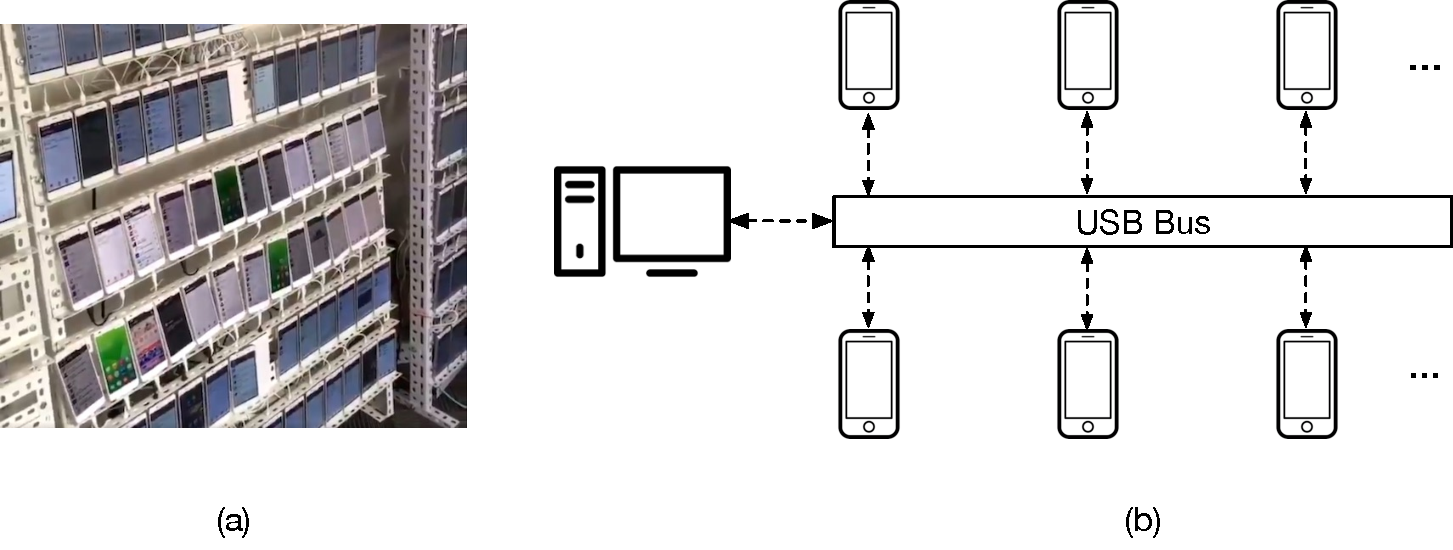
\includegraphics[width=0.44\textwidth]{Figures/clickfarm}
	\caption{(a) A photo inside a real-life click farm \cite{clickphoto}. (b) The general set up of a click farm, where phones are powered up and connected to a central server via USB connections. }
	\label{fig:clickfarm}
	\end{center}
	\end{figure}
	However, despite the effectiveness, 
	setting up such a farm incurs a substantial cost. The major expenses is for purchasing the massive number of devices. Meanwhile, the subsequent deployment and maintenance tasks also involve huge labor costs.
	These drawbacks naturally inspire us to investigate the potential of replacing the physical devices with device emulators. Device emulators are in essence virtual machines that are mainly designed for developers to swiftly prototype mobile applications without using hardware devices. Compared with physical devices, emulators are significantly more cost-effective because they can be massively deployed in cloud platforms or local servers in a cheap price. For instance, the average price for a low-end smartphone with one-year lifespan is approximately 215 USD \cite{pricesmartphone}, while the money can enable us to host 6 emulator instances without optimization in the cloud for a same timespan \cite{vpscom}. Besides, deploying and maintaining emulators is less labor intensive owning to existing automated management systems \cite{mutti2015baredroid}.

	Though the idea of launching click fraud with emulators seems quite straightforward, practical implementation entails substantial challenges. 
	First, existing device emulators are CPU-intensive and memory-intensive. It likely results in poor performance and application failure due to resource constraints. Moreover, the high resource demand also decreases the number of emulator instances that can be run concurrently, which limits the power of the attack. % Meanwhile, it inevitably  . 
	% In other words, it reduces the scale of an attack with a limited budget. 
	Second, the existing emulators are easily blocked by various mobile applications due to their defective device profiles. A profile serves as a unique device signature, usually consisting of properties such as WiFi MAC addresses or phone numbers that are hardware-specific. Since the corresponding hardware components are not emulated, the property values remain empty. Therefore, by scrutinizing the defective device profile, an application can easily identify and block the emulator.
	% each mobile application account, in order to remain active, is required to associate with a unique hardware-related device profile.
	Finally, it is challenging to deploy and manage numerous emulator instances in a large-scale attack, because existing emulator management systems are centralized and they fail to cope with the scale-out and fault tolerance issues. 

	 
	% The high resource usage greatly decreases the number of emulator instances that can be run concurrently given certain cloud resources. 
	% Specifically, existing emulators are mainly designed for developers to swiftly prototype and test Android applications without using hardware devices. 
	% They lack several important features required by a successful large-scale attack.

	% First, the emulators only provide limited or even no emulation for some hardware components of a real device (e.g., a cellular modem). It renders some important functionalities such as receiving text messages and dialing a phone call unusable in an emulator. However,  these functionalities are indispensable when launching attacks on a great number of mobile applications guarded by text message verification. It require a device to have a genuine phone number and be able to receive text messages for verification codes before certain actions are granted (e.g., registration or posting). 


	In this paper, we propose Fraus, a novel approach that enables individuals to launch MCFA using device emulators. Specifically, Fraus significantly reduces CPU usage by circumventing the compute-intensive graphics emulation. It also maintains a small memory footprint by applying the lazy-loading and deduplication techniques on system components. To bypass device-profile scrutiny, Fraus implements two virtual hardware components including cellar modems and WiFi interfaces. They enable each emulator instance to generate a seemingly authentic device profile. Meanwhile, Fraus offers a distributed emulator cluster management system, which is scalable, fault-tolerant and easy-to-use. Its API abstraction features a logically centralized view, which allows an user to easily program and launch an attack task without concerning the details of the underlying distributed protocols.
	% A memory isolation mechanism is also introduced to allow multiple applications to run on a same instance 

	We consolidate the above techniques and implement the prototype of Fraus on top of Android 6.0. We conduct comprehensive experiments to evaluate Fraus against the top 300 applications from the Google Play store. Experimental results show that Fraus has high application compatibility and system stability because 96\% of the selected applications run successfully, while the number is only 59\% for existing emulators. Fraus also reduces CPU usage and memory footprint up to 90\% and 60\% respectively compared with the existing emulators. The small resource demand enables fitting 125 instances in a low-end server equipped with 32GB RAM, reflecting the high cost efficiency.
	% All the applications run smoothly on Fraus, indicating its high system stability. A cluster consisting 500 virtual devices is also set up to demonstrate the Fraus's scalability.
	% \textbf{Rephrase it! And add countermeasure, make it politically correct.}

	To the best of our knowledge, Fraus is the first system that is designed to launch a cost-efficient and scalable MCFA via devices emulators. By designing Fraus, we aim to raise public concerns about the simplicity of committing click fraud and to suggest countermeasures to mitigate such risks.

	% The main contributions of this paper are as follows:
	% \begin{enumerate}
	% \item We present approaches to circumvent CPU-intensive display emulation and to reduce memory usage without affecting system stability.
	% \item We implement a set of virtual devices and drivers that enable an emulator to generate a unique device profile. \textbf{Rephrase it ! And add countermeasure}
	% \item We conduct experiments to confirm the high performance and scalability of our prototype. 
	% \end{enumerate}

	 % Specifically, to bypass text message verification, Fraus utilizes a custom-tailored Android emulator, which emulates the text-messaging and phone dialing functionalities with the help of on-line virtual phone services.  Besides, to keep a tiny memory footprint (around 130 Mb), Fraus carefully prunes a great number of non-essential Android system services while making sure the system stability in not affected. Fraus only requires a small CPU processing power as it avoids the most compute-intensive emulation of video display and audio playback. Meanwhile, Fraus also utilizes a elastically scalable network architecture that automatically deploys and manages the emulator instances in popular cloud services.  

	% The emulator instances along with the automation scripts then will be automatically deployed to popular cloud services 

	% After composing the automation scripts, the emulators will be automatically deployed in a elastically scalable network architecture residing in remote cloud. 

	% We should talk about some experiments?

	The rest of this paper is organized as follows. Section.~\ref{motivate} investigates the problems of launching MCFA using existing emulators.
	% Section.~\ref{overview1} overviews the architecture design and the key components of Fraus.
	Section.~\ref{Circuvment} presents the approach to disable the compute-intensive graphics emulation. Section.~\ref{memory} describes optimization techniques that reduce the memory footprint. Section.~\ref{deviceid} illustrates the methodology to bypass device profile scrutiny. Section.~\ref{deploymentarch} elaborates the architecture for the distributed emulator instance management system.  Section.~\ref{expm} reports the evaluation results. Section.~\ref{countermeasure} discusses the countermeasures to combat Fraus. Section.~\ref{related} surveys the related work and Section.~\ref{conclusion} concludes this paper.


	\section{Background and Motivation}\label{motivate}
	Little research has been conducted to investigate the usability of emulators on MCFA. 
	In this section, we attempt to evaluate the usability and identify the potential problems pending to be addressed via preliminary experiments.
	% In this section, we conduct some preliminary studies by 
	% A click fraud attack can be roughly separated into two essential stages; the first step is to register a scam account and the second step is to repeatedly generate click events with the account. Take Facebook as an example, the malicious will by all means register a huge number of the application accounts and automate them to generate phoney 'likes' by clicking the 'thumb' button. 
	We first select 4 target mobile applications from two genres that are frequent victims of MCFA, including social media and online advertising. The selected social media applications consist of \textit{Facebook} and \textit{Wechat}. The selected online advertising applications, which reward users for every view of a commercial video clip, include \textit{Daily Cash} and \textit{Lucky Cash}.
	We run these applications on three widely-used options including \textit{Android Official Emulator} \cite{andemu}, \textit{BlueStacks} \cite{bluestack} and \textit{GenyMotion} \cite{genymotion}. These emulators are allocated with an one-core 2.2 GHz virtual CPU, 512 MB RAM, and 12 MB video RAM with GPU acceleration disabled. This resource configuration is chosen to be close to the specification of a low-end virtual machine provided by most cloud platforms \cite{vpscom}. In our mocking attack, we identify the following difficulties.

	\textbf{Performance Issues.} The first difficulty arises from the performance issues of emulators. We observe that the emulators tend to be CPU-intensive. 
	To demonstrate our observation, we measure the average system-wide CPU usage when the emulators are automated to perform predefined tasks such as clicking a like button or viewing a video clip in the 4 applications. The results are shown in Table~\ref{tab:precpu}. It can be seen that 
	all the applications are incurring high CPU workload regardless of the types of emulators. Specifically, the social media applications consume almost half of the CPU processing power. The advertising applications appear to be more compute-intensive and nearly saturate the CPU. 

	To pinpoint the root cause of high system-wide CPU utilization, we further demonstrate the usage of each running process in an emulator in Table~\ref{processcpu}. Note that we only list the CPU statistics for the Android official emulator because different emulators yield similar CPU performance. One essential finding from the table is that although the overall CPU usage is high, only a small proportion is attributed to the application itself. Two system processes \textit{Surfaceflinger} and \textit{Mediaserver} are the main culprits of the excessive CPU usage. Surfaceflinger is an Android system service, in charge of compositing graphical user interfaces (GUI) of applications into a single buffer, which is finally displayed by a screen. Mediaserver is another important system service that entitles an application to play various types of video files. The two system services involve a great amount of graphical computation, which can be offloaded to GPUs in physical devices. However, GPUs are not available in an emulator and the graphical computation has to be conducted by CPUs inefficiently,  which justifies the high CPU workload of the Surfaceflinger and Mediaserver.

	% The two system services are the core components of the Android graphics system. In a physical device,  

	%
	% the CPU consumption does not significant differ regardless of the emulators being used. Therefore, it allows us to conduct the remaining analysis on just one type of emulator.

	\begin{table}[t]
	\centering
	\footnotesize
	\caption{System Wide CPU Usage When Running Selected Applications.}
	\label{tab:precpu}
	\setlength\tabcolsep{10pt}
	\begin{tabular}{|l|l|l|l|}
	\hline
	CPU Usage  & Offical & BlueStack & GenyMotion \\ \hline
	Wechat     & 43\%    & 47\%      & 45\%       \\ \hline
	Facebook   & 57\%    & 54\%      & 59\%       \\ \hline
	Daily Cash & 79\%    & 76\%      & 78\%       \\ \hline
	Lucky Cash & 87\%    & 83\%      & 84\%       \\ \hline
	\end{tabular}
	\vspace{-0.2in}
	\end{table}
	% \begin{figure}[ht]
	% \begin{center}
	% 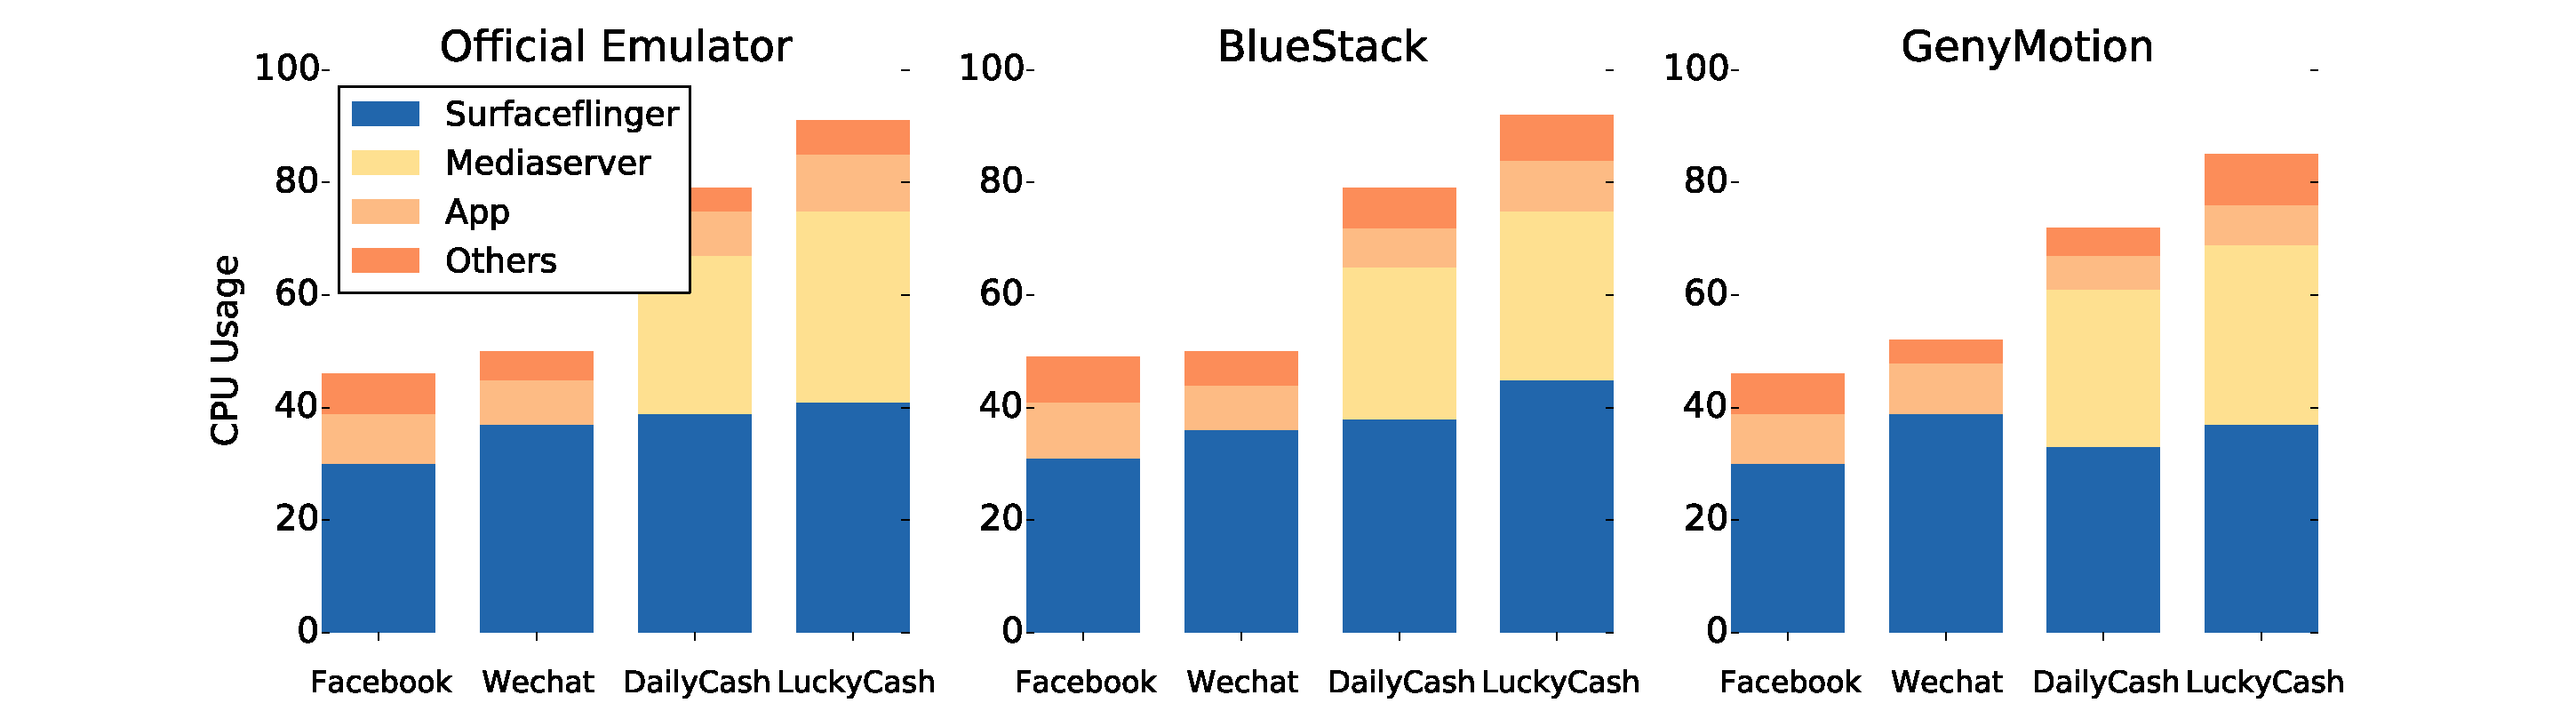
\includegraphics[width=0.50\textwidth]{Figures/precpu}
	% \caption{Typical system deployment.}
	% \label{fig:precpu}
	% \end{center}
	% \end{figure}

		
		\begin{table}[t]
		\footnotesize
		\centering
		\caption{CPU utilization of each running process in an emulator.}
		\label{processcpu}
		\setlength\tabcolsep{0.4pt}
		\begin{tabular}{|l|l|l|l|l|l|}
		\hline
		CPU Usage  & Surfaceflinger & Mediaserver & Systemservice & App. itself & Others \\ \hline
		Wechat     & 25\%           & 0\%         & 3\%           & 11\%        & 4\%    \\ \hline
		Facebook   & 37\%           & 2\%         & 4\%           & 13\%        & 1\%    \\ \hline
		Daily Cash & 11\%           & 49\%        & 7\%           & 7\%         & 5\%    \\ \hline
		Lucky Cash & 23\%           & 43\%        & 5\%           & 10\%        & 6\%    \\ \hline
		
		\end{tabular}
		\vspace{-0.1in}
		\end{table}
			
	%  and it can be
	% seen that regarding the official Android emulator, it occupies full CPU power regardless of the applications are running. Even that, the running applications are still suffering from noticeable lag. On the other hand, the GenyMotion emulator consumes significantly less CPU power when executing social media applications. However, advertisement applications still exhaust a huge portion of CPU capacity.

	Another performance concern is the excessive memory usage. The minimum memory requirement of BlueStack and GenyMotion is 2 GB. It means that the only way to run them in the virtual machine with 512 MB RAM is to enable swapping. However, swapping may negatively impact the system performance due to the potential thrashing behavior. The Android official emulator somehow possesses a smaller footprint, which is approximately 500 MBs right after the system starts up. Nevertheless, the free RAM is extremely limited and swapping is still required in order to run any other applications. 
	 % We examine the memory statistics by using the \textbf{PS} command. We notice that a process name \textbf{system\_server} consumes a huge amount of memory (around 127 MB) 

	% It is clear to see that given certain computational resources, the extensive CPU usage and memory footprint could greatly reduce the number of emulators that can be run concurrently. It then limits the scale of the attack that an attacker can carry out. 

	\textbf{Defective Device Profile.} We meet the second obstacle when running applications that enforce device profile scrutiny. A device profile serves as a unique device identification. It usually consists of several hardware-specific properties. Commonly used properties include:
	\begin{enumerate}
	\item WiFi Media Access Control (MAC) Address, a unique identifier assigned to WiFi interfaces.
	\item The cell phone number of the device.
	\item International Mobile Subscriber Identity (IMSI), a unique number to identify the user of a cellular network.
	\item International Mobile Equipment Identity (IMEI), a unique 15-digit serial number given to every mobile phone's cellular modem.
	\end{enumerate}
	All the properties are retrieved from hardware components including cellular modems and WiFi interfaces. Since they are not emulated,  the above property values remain empty in an emulator. The artifact then allows application providers to easily identify and block the emulators. To make matters worse, the authenticity of the properties, especially the phone number, can be easily verified by the applications. For instance, many applications send the number a SMS containing verification codes to ensure the number is genuine. It makes randomly generating the property values an infeasible approach to bypass the scrutiny.


	% only regard a view as an authenticated one when the device's profile is currently associated with one account. Since all emulators share one dummy profile, if we sign in various accounts in different emulators, we could easily breach the criteria.
	% To defeat scam accounts, all the mobile applications we are testing have implemented text-message verification. It requires a user to have a genuine phone number and be able to receive text messages for verification codes before the registration can be finished. However, the existing emulators only provide limited or even no emulation for the cellular network modem, rendering the indispensable functionalities such as receiving text messages and dialing a phone call unusable. In other words, the existing emulators are not able to bypass the text-message verification.

	% We also notice that some applications further adopt Device-ID verification to prevent attackers from registering scam accounts. During the registration process, the applications will note down some device-specific information. Usually, it contains Media Access Control (MAC) addresses of bluetooth and WiFI interfaces. The information is theoretically unique for every smart device and can be used as a device-id. The device-id verification  will usually enforce every newly registered-account should be associated with a never-seen device-id.  Therefore, the emulators are not able to bypass the Device-ID verification.

	
	\section{Conclusion}\label{conclusion}
	In this paper, we raise public concerns of the simplicity of launching a large-scale MCFA by presenting Fraus. Fraus has a tiny CPU and memory resource demand. Besides, Fraus can generate a seemingly authentic device profile and disguise itself as a legitimate device. To facilitate a large-scale attack, Fraus also provides a distributed emulator cluster management system, which is scalable and fault-tolerant. We evaluate the performance of Fraus and demonstrate that Fraus has high application compatibility and cost efficiency. Finally, we also propose countermeasures leveraging Fraus's platform-specific characteristics to combat such an attack.

	\begin{spacing}{0.8} 

	\bibliographystyle{IEEEtran}
	\bibliography{myrefs}
	\end{spacing}
	\end{document}

